\subsection{Overview}
As stated above, the system is divided into three subsystems, which are represented in the following figure.

\FloatBarrier

\begin{figure}[!h]
	\centering
	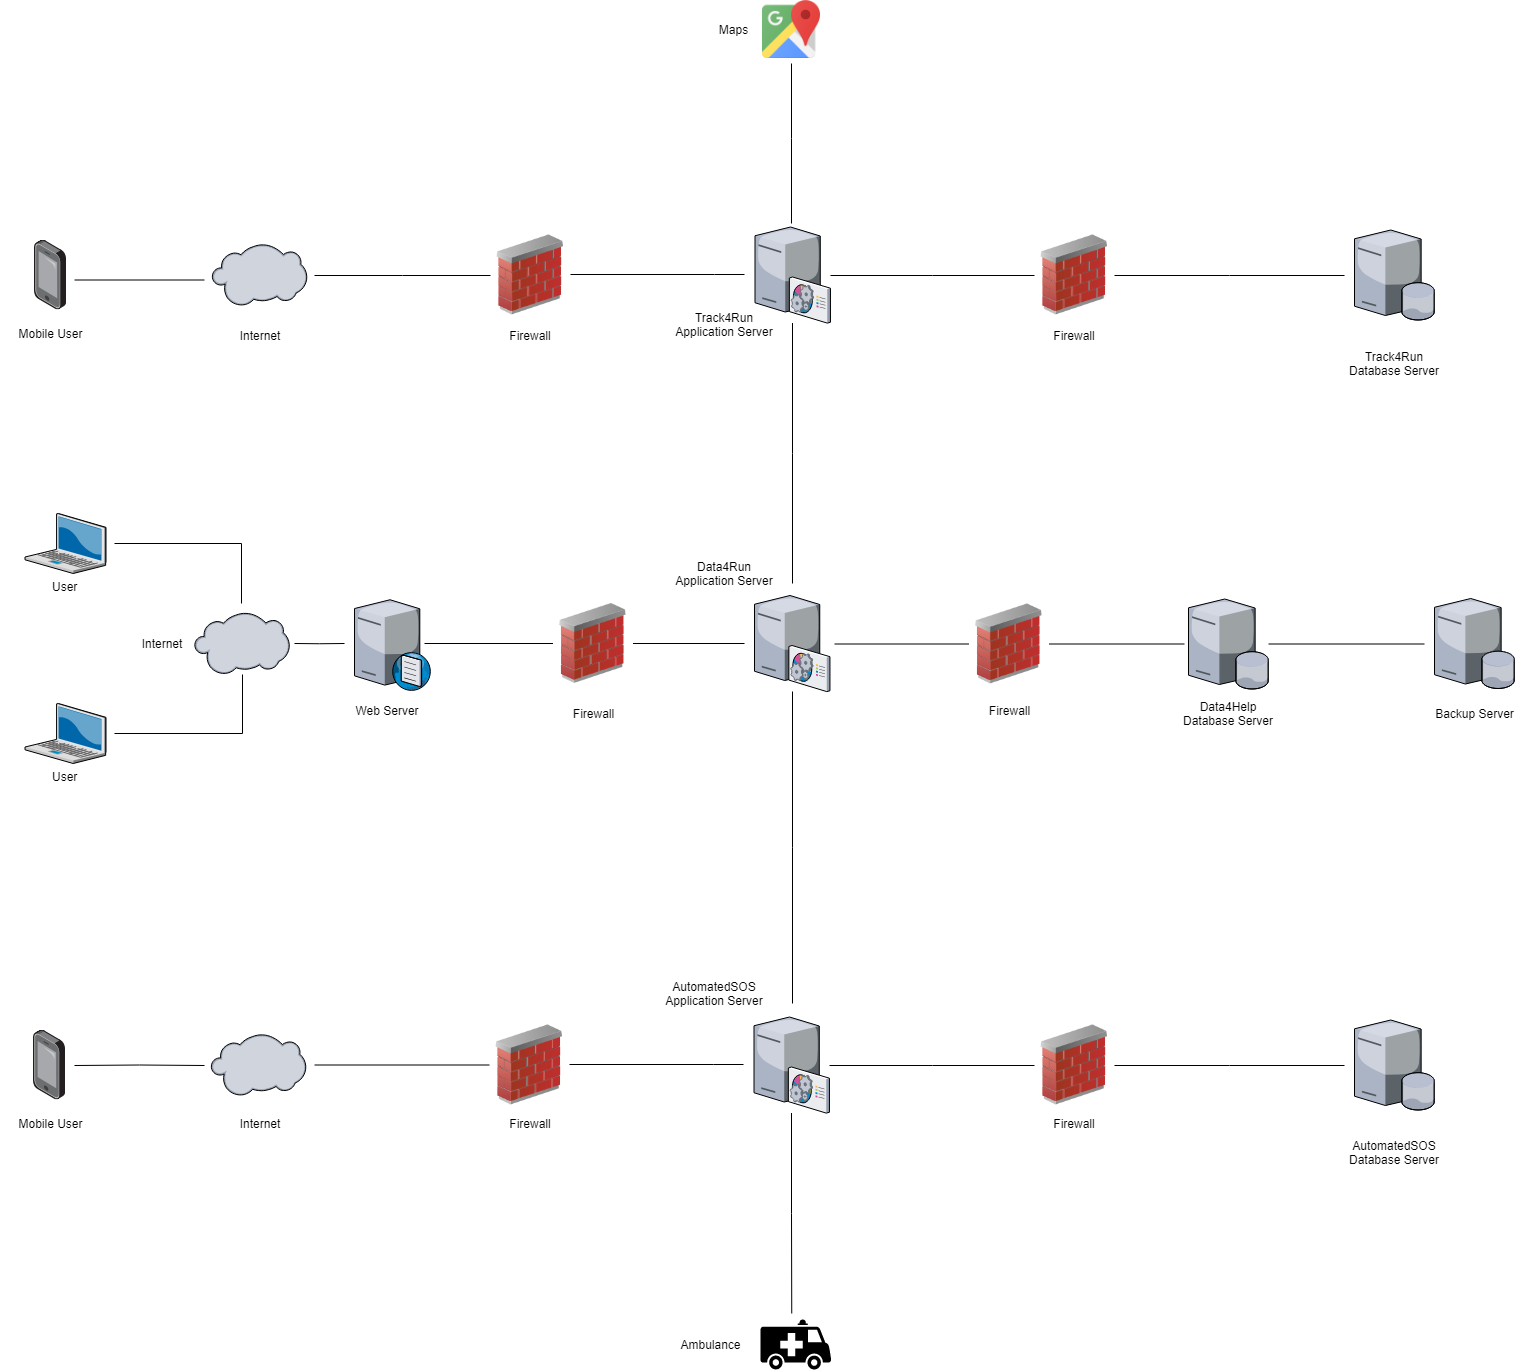
\includegraphics[width=\columnwidth]{physicalArchitectureDiagram.png}
	\caption{General Architecture}
\end{figure}


\FloatBarrier

In particular, Data4Help subsystem can be accessed via browser by users and third parties, but also using the dedicated APIs (for data-sources and third parties). It is designed as a three-tier application with a thin browser client and a thick back-end, in which data processing, protection and storage are critical functions.

AutomatedSOS and Track4Run instead are designed as applications with a thick client (i.e. smart-phone and smart-watch apps), a lightweight back-end server and a storage module. This design has been chosen because it is completely modular on one hand, since the two application's business logic is separated from Data4Help's one, but guarantees on the other hand a fast and reliable service provided by the servers, leaving the full responsibility of the presentation part to the mobile application. This separation also guarantees a good maintainability of the system and good performances on the mobile side, where power consumption and CPU usage can be an issue.

\subsection{High Level Architecture}

\FloatBarrier
\begin{figure}[!h]
	\centering
	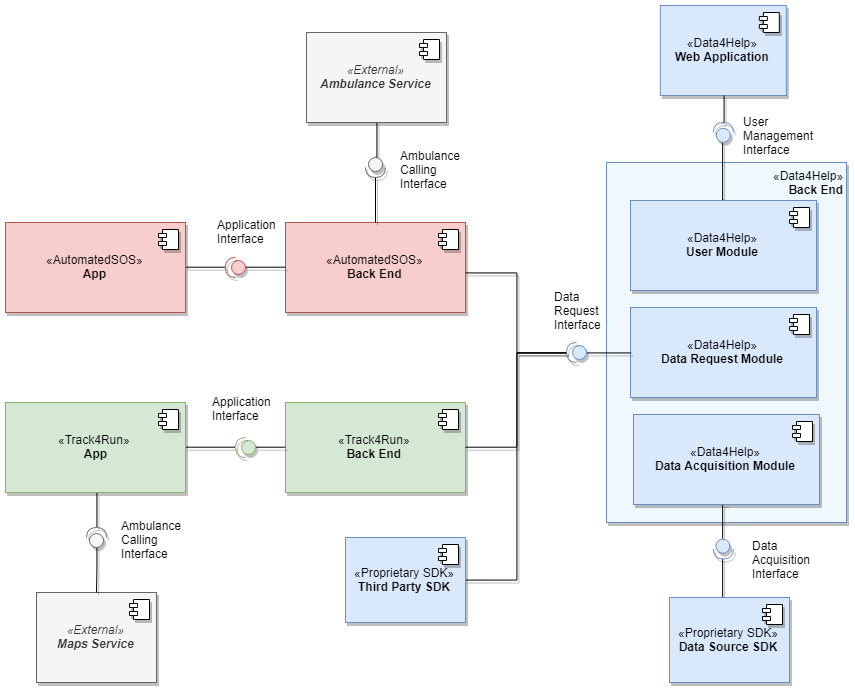
\includegraphics[width=\columnwidth]{ComponentDiagrams-Total.png}
	\caption{High Level Components}
\end{figure}

\FloatBarrier


\subsection{Component View}


\begin{itemize}
	\item \textbf{Data4Help}
\end{itemize}

\FloatBarrier
\begin{figure}[!h]
	\centering
	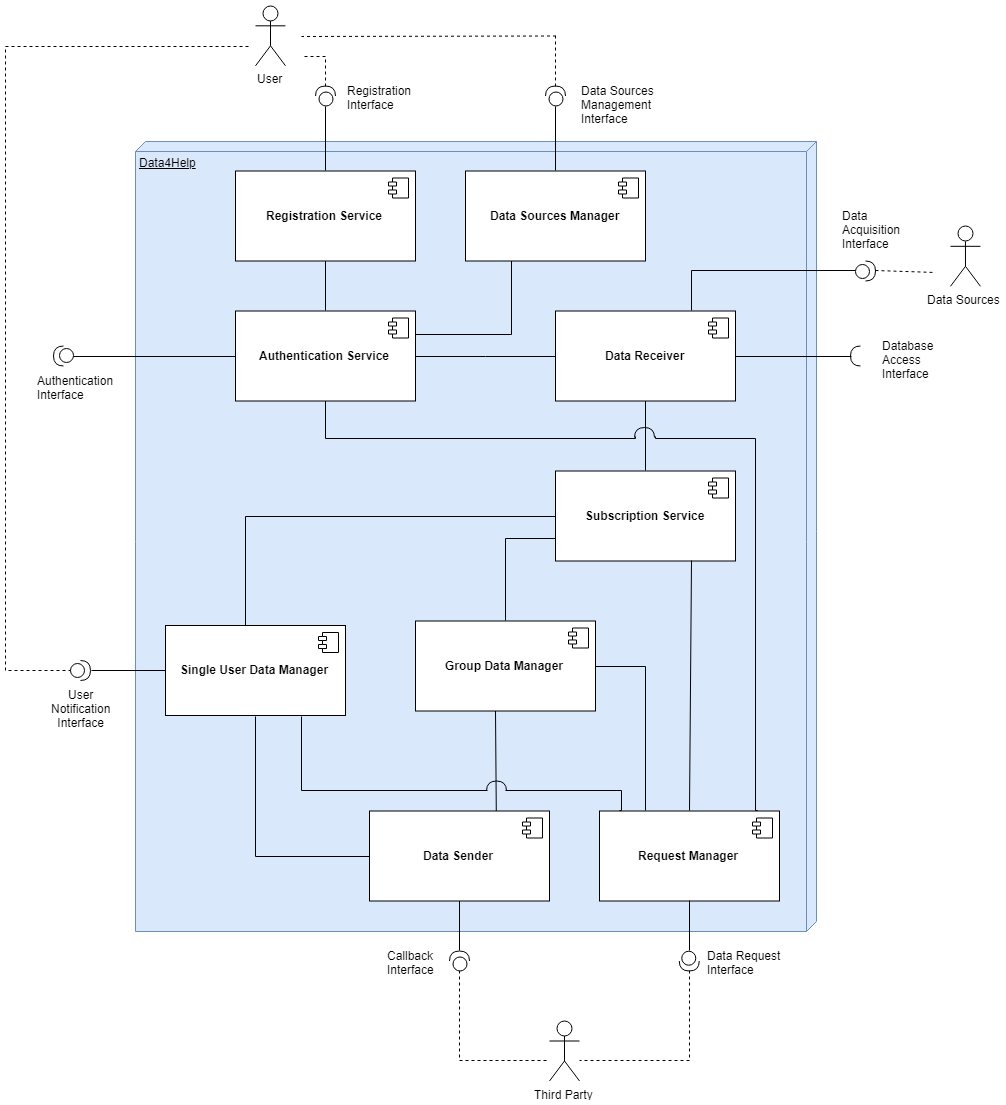
\includegraphics[width=\columnwidth]{ComponentDiagrams-Data4Help.png}
	\caption{Data4Help Components}
\end{figure}

\FloatBarrier



\begin{itemize}
	\item \textbf{AutomatedSOS}
\end{itemize}

\begin{figure}[!h]
	\centering
	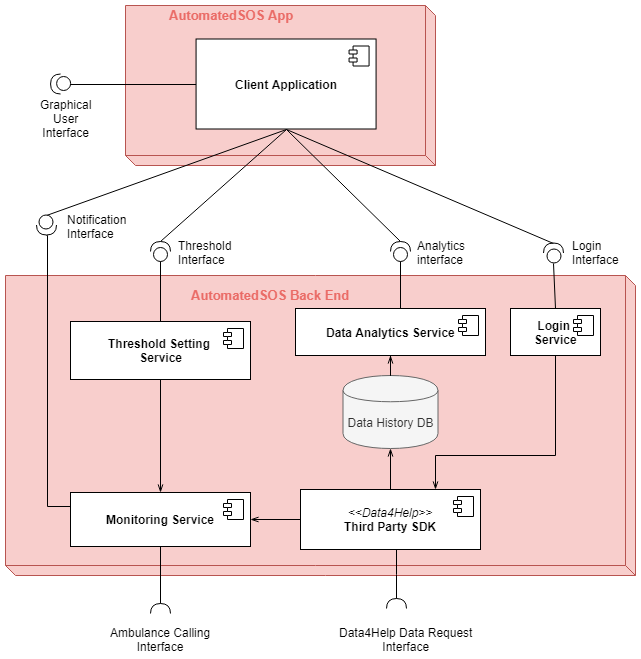
\includegraphics[width=\columnwidth]{ComponentDiagrams-AutoSOS.png}
	\caption{AutomatedSOS Components}
\end{figure}

\FloatBarrier



\begin{itemize}
	\item \textbf{Track4Run}
\end{itemize}

\FloatBarrier
\begin{figure}[!h]
	\centering
	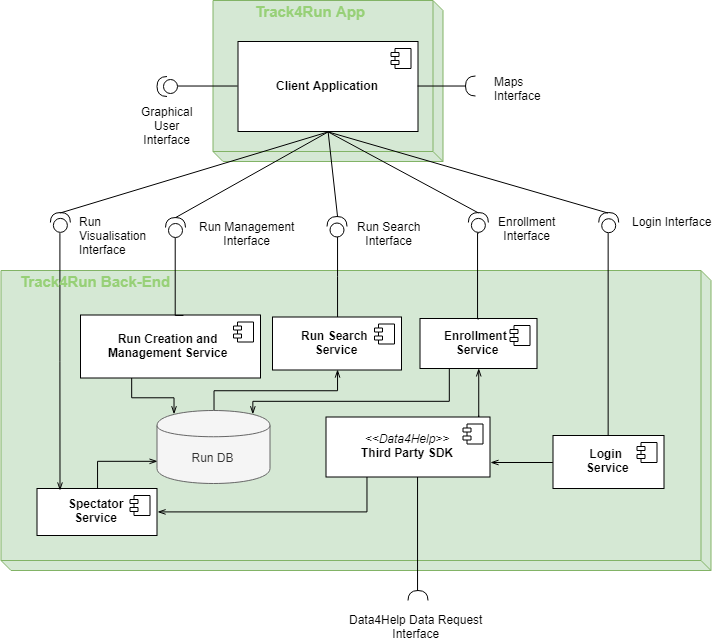
\includegraphics[width=\columnwidth]{ComponentDiagrams-Track4Run.png}
	\caption{Track4Run Components}
\end{figure}

\FloatBarrier


\subsection{Deployment View}
\subsection{Runtime View}
\subsection{Component Interfaces}
\subsection{Selected Architectural Styles and Patterns}
\subsection{Other Design Decisions}